\section{Tall-and-Skinny QR}
\label{sec:TSQR}
	Some important problems that require QR factorizations of overdetermined systems include least squares problems, eigenvalue problems, low rank approximations, as well as other matrix decompositions.
	Although Tall-and-Skinny QR (TSQR) broadly refers to row-block QR factorization methods, we will discuss a specific variant of TSQR which is also known as the AllReduce algorithm \cite{Mori2012}.
	In this paper, the TSQR/AllReduce algorithm refers to the most parallel variant of all row-block QR factorization algorithms discussed in \cite{Demmel2012}.
	A detailed description and rounding error analysis of this algorithm can be found in \cite{Mori2012}, and we present a pseudocode for the algorithm in Algorithm~\ref{algo:par_tsqr}.
	Our initial interest in this algorithm came from its parallelizable nature, which is particularly suitable to implementation on GPUs. 
	Additionally, our numerical simulations (discussed in Section~\ref{sec:NE}) show that TSQR can not only increase the speed but also outperform the traditional HQR factorization in low precisions.
	\subsection{TSQR/AllReduce Algorithm}
		Algorithm~\ref{algo:par_tsqr} takes a tall-and-skinny matrix, $\bb{A}$, and organizes it into row-blocks. 
		HQR factorization is performed on each of those blocks, and pairs of $\bb{R}$ factors are combined  to form the next set of $\bb{A}$ matrices to be QR factorized. 
		This process is repeated until only a single $\bb{R}$ factor remains, and the $\bb{Q}$ factor is built from all of the Householder constants and vectors stored at each level.
		The most gains from parallelization can be made in the initial level where the maximum number of independent HQR factorizations occur. 
		Although more than one configuration of this algorithm may be available for a given tall-and-skinny matrix, the number of nodes available and the shape of the matrix eliminate some of those choices. 
		For example, a 1600-by-100 matrix can be partitioned into 2, 4, 8, or 16 initial row-blocks but may be restricted by a machine with only 4 nodes, and a 1600-by-700 matrix can only be partitioned into 2 initial blocks.
		%The choice in the initial partition determine the recursion depth which we call level.
		Our numerical experiments show that the choice in the initial partition, which directly relates to the recursion depth of TSQR, has an impact in the accuracy of the QR factorization. \par
		%Our numerical experiments provide some insight into how to make this decision in an optimal way.  \par
		
		We refer to \emph{level} as the number of recursions in a particular TSQR implementation. 
		An $L$-level TSQR algorithm partitions the original matrix into $2^L$ submatrices in the initial or $0^{th}$ level of the algorithm, and $2^{L-i}$ QR factorizations are performed in level $i$ for $i = 1 , \cdots, L$. 
		The set of matrices that are QR factorized at each level $i$ are called $\bb{A}_j^{(i)}$ for $j = 1, \cdots, 2^{L-i}$, where superscript $(i)$ corresponds to the level and the subscript $j$ indexes the row-blocks within level $i$.
		%Note that each $\bb{A}_i^{(j)}$ is created from combining two $\bb{R}$ factors in the previous level, $i-1$.
		%,  $\bb{A}$ matrices that are QR factorized.
		%The initial row-blocks that partition the original matrix is the initial or $0^{th}$ level of the algorithm, and each successive set of $\bb{A}_i^{(j)}$ matrices (created from combining $\bb{R}$ factors of the previous level) are referred to as first level, second level, and so forth.
		%The subscript, $i$ corresponds to the level, and the superscript $(j)$ indexes the row-blocks within level $i$.
		In the following sections, Algorithm~\ref{algo:par_tsqr} ({\tt tsqr}) will find a TSQR factorization of a matrix $A\in\R^{m\times n}$ where $m \gg n$. 
		The inline function {\tt qr} refers to Algorithm~\ref{algo:hhQR}, {\tt hh\_mult} is Algorithm~\ref{algo:hh_mult}, and we use Algorithm ~\ref{algo:hh_v2} as a subroutine of {\tt qr}.

%		performs a HQR factorization and returns $\bb{V} \in \R^{m\times n}$, $\bm{\beta}\in\R^{n}$, and $\bb{R} \in R^{n\times n}$.
%		For $i=1,\cdots,n$, the $i^{th}$ column of $\bb{V}$ and $\bm{\phi}_i$ are the Householder vector and constant that defines the $i^{th}$ Householder transformation matrix, $\bb{P}_i$ for the QR decomposition of the input matrix. 
%		The columns of $\bb{V}$ are the Householder vectors (first component normalized to $1$) that can form the matrix $\bb{Q}_{\text{thin}} = \bb{P}_1 \cdots \bb{P}_nI_{m\times n}$.
%		Note that a full $\bb{Q}$ can be constructed via $\bb{Q}_{\text{full}}=\bb{P}_1\cdots \bb{P}_n$. 
%		
%		
%		Algorithm~\ref{algo:hh_mult} is the implementation of multiplying  $\bb{Q}:= \bb{P}_1 \cdots \bb{P}_n$ to another matrix or vector, when only the householder vectors to construct $\bb{P}_i$'s are given. This takes advantage of the special property of householder matrices-- $\bb{P}_i$'s are rank-one updates of the identity. let $\bb{B}\in\R^{m\times d}$. The straightforward mod of  computing $\bb{Q}\bb{B}$ costs $\mathcal{O}(m^2d)$ where the costs of constructing $\bb{Q}$ itself is ignored. However,  Algorithm ~\ref{algo:hh_mult} describes a method that is only $\mathcal{O}(mnd)$. 

		\subsubsection{TSQR Notation}
		We will introduce new notation due to the multi-level nature of the TSQR algorithm.
		In the final task of constructing $\bb{Q}$, $\bb{Q}_j^{(i)}$ factors are aggregated from each block at each level.
		Each $\bb{Q}_j^{(i)}$ factor from level $i$ is partitioned such that two corresponding $\bb{Q}^{(i-1)}$ factors from level $i-1$ can be applied to them. 
		The partition (approximately) splits $\bb{Q}_{j}^{(i)}$ into two halves, $[\tilde{\bb{Q}}_{j, 1}^{(i)\top} \tilde{\bb{Q}}_{j, 2}^{(i)\top}]^{\top}$.
		% \(\bb{Q}_{j}^{(i)} = \begin{bmatrix}
		%\tilde{\bb{Q}}_{j, 1}^{(i)}\\ 
		%\tilde{\bb{Q}}_{j, 2}^{(i)} 
		%\end{bmatrix},\)
		The functions $\alpha(j)$ and $\phi(j)$ are defined such that $\bb{Q}_j^{(i)}$ is applied to $\tilde{\bb{Q}}_{\alpha(j), \phi(j)}^{(i+1)}$.
		For $j = 1 , \cdots, 2^{L-i}$ at level $i$, we need $j = 2(\alpha(j)-1) + \phi(j)$, where $\alpha(j) = \lceil \frac{j}{2}\rceil$ and $\phi(j) = 2 + j - 2\alpha(j)$.
%		\begin{itemize}
%			\item $\alpha(j) = \lceil \frac{j}{2}\rceil $ and
%			\item $\phi(j) = 2 + j - 2\alpha(j)$.
%		\end{itemize} 
		Section~\ref{Qdetails} shows full linear algebra details for a single-level ($L=1$, $2$ initial blocks) example.
		The reconstruction of $\bb{Q}$ can be implemented more efficiently (see \cite{BDGJNS2014}), but the reconstruction method in Algorithm~\ref{algo:par_tsqr} is presented for a clear, straightforward explanation.
		
		\subsubsection{Single-level Example}
		\label{Qdetails}
		In the single-level version of this algorithm, we first bisect $\bb{A}$  into $\bb{A}_1^{(0)}$ and $\bb{A}_2^{(0)}$ and compute the QR factorization of each of those submatrices.
		We combine the resulting upper-triangular matrices , i.e.,  \(\bb{A}_{1}^{(1)} =\begin{bmatrix}
		\bb{R}_{1}^{(0)}\\ 
		\bb{R}_{2}^{(0)} 
		\end{bmatrix},\)   which is QR factorized, and the process is repeated:
		\[
		\bb{A} = \begin{bmatrix}
		\bb{A}_1^{(0)}\\
		\bb{A}_2^{(0)}
		\end{bmatrix} = \begin{bmatrix}
		\bb{Q}_1^{(0)}\bb{R}_1^{(0)}\\
		\bb{Q}_2^{(0)}\bb{R}_2^{(0)}
		\end{bmatrix} = \begin{bmatrix}
		\bb{Q}_1^{(0)} & \bb{0}\\
		\bb{0} & \bb{Q}_2^{(0)}
		\end{bmatrix} \begin{bmatrix}
		\bb{R}_1^{(0)} \\
		\bb{R}_2^{(0)}
		\end{bmatrix} =\begin{bmatrix}
		\bb{Q}_1^{(0)} & \bb{0}\\
		\bb{0} & \bb{Q}_2^{(0)}
		\end{bmatrix} \bb{A}_1^{(1)} =\begin{bmatrix}
		\bb{Q}_1^{(0)} & \bb{0}\\
		\bb{0} & \bb{Q}_2^{(0)}
		\end{bmatrix} \bb{Q}_1^{(1)}\bb{R}.%_1^{(1)}
		\] 
		The $\bb{R}$ factor of $\bb{A}_1^{(1)}$ is the final $\bb{R}$ factor of the QR factorization of the original matrix, $\bb{A}$. 
		However, the final $\bb{Q}$ still needs to be constructed.
		Bisecting  $\bb{Q}_1^{(1)}$ into two submatrices, i.e. $\tilde{\bb{Q}}_{1,1}^{(1)}$ and $\tilde{\bb{Q}}_{1,2}^{(1)}$, allows us to write and compute the product more compactly,  \[
	    \bb{Q}:=\begin{bmatrix}
		\bb{Q}_1^{(0)} & \bb{0}\\
		\bb{0} & \bb{Q}_2^{(0)}
		\end{bmatrix} \bb{Q}_1^{(1)} =    \begin{bmatrix}
		\bb{Q}_1^{(0)} & \bb{0}\\
		\bb{0} & \bb{Q}_2^{(0)}
		\end{bmatrix} \begin{bmatrix}
		\tilde{\bb{Q}}_{1,1}^{(1)}\\
		\tilde{\bb{Q}}_{1,2}^{(1)}
		\end{bmatrix}= \begin{bmatrix}
		\bb{Q}_1^{(0)}\tilde{\bb{Q}}_{1,1}^{(1)} \\ 
		\bb{Q}_2^{(0)}\tilde{\bb{Q}}_{1,2}^{(1)}
		\end{bmatrix}. \]
		More generally, Algorithm~\ref{algo:par_tsqr} takes a tall-and-skinny matrix $\bb{A}$ and level $L$ and finds a QR factorization by initially partitioning $\bb{A}$ into $2^L$ row-blocks and includes the building of $\bb{Q}$.
		
		\begin{algorithm2e}[H]
			\DontPrintSemicolon % Some LaTeX compilers require you to use \dontprintsemicolon instead
			\KwIn{$\bb{A}\in\R^{m \times n}$ where $m \gg n$, $L\leq\lfloor\log_2\left(\frac{m}{n}\right)\rfloor$, and $2^L$ is the initial number of blocks. }
			
			\KwOut{$\bb{Q}\in\R^{m \times n}$, $\bb{R} \in\R^{n\times n}$ such that 	$\bb{Q}\bb{R} = \bb{A}$.}
			$h \gets \lfloor \frac{m}{2^L} \rfloor$ \tcp*{Number of rows for all but the last block.}
			$r \gets m - (2^L-1)h$ \tcp*{Number of rows for the last block ($h\leq r <2h$).}
			\tcc{Split $\bb{A}$ into $2^L$ blocks. Note that level $(i)$ has $ 2^{L-i}$ blocks.}
			\For {$j = 1 : 2^L-1$}{
				$\bb{A}_j^{(0)} \gets \bb{A}[(j-1)h+1: jh, :]$ %\bb{I}_{(j-1)h, jh}^{\top}\bb{A}$
			}
			$\bb{A}_{2^L}^{(0)} \gets \bb{A}[(2^L-1)h:m, :]$ \tcp*{Last block may have more rows.} %\bb{I}_{(2^L-1)h, m}^{\top}\bb{A}
			\tcc{Store Householder vectors as columns of matrix $\bb{V}_j^{(i)}$, Householder constants as components of vector $\bm{\beta}_j^{(i)}$, and set up the next level.}
			\For{$i = 0 : L-1$}{
				\tcc{The inner loop can be parallelized.}
				\For {$j = 1 : 2^{L-i}$ }{
					$\bb{V}_{2j-1}^{(i)}$, $\bm{\beta}_{2j-1}^{(i)}$, $\bb{R}_{2j-1}^{(i)} \gets{\tt qr}(\bb{A}_{2j-1}^{(i)})$ \;
					$\bb{V}_{2j}^{(i)}$, $\bm{\beta}_{2j}^{(i)}$, $\bb{R}_{2j}^{(i)} \gets{\tt qr}(\bb{A}_{2j}^{(i)})$\;
					% \tcp*{$\bb{V}_j^{(i)} \in \R^{2n\times n}$ for $i > 0$ and $\bb{R}_j^{(i)} \in \R^{n\times n}$ always.} 
					\(\bb{A}_{j}^{(i+1)} \gets \begin{bmatrix}
					\bb{R}_{2j-1}^{(i)}\\
					\bb{R}_{2j}^{(i)}
					\end{bmatrix}\)
				}
			}
			\tcc{At the bottom-most level, get the final $\bb{R}$ factor.}
			$\bb{V}_{1}^{(L)}$, $\bm{\beta}_1^{(L)}$, $\bb{R}  \gets{\tt qr}(\bb{A}_{1}^{(L)})$ \;
			$\bb{Q}_{1}^{(L)} \gets {\tt hh\_mult}(\bb{V}_{1}^{(L)}, I_{2n\times n})$\;
			\tcc{Compute $\bb{Q}^{(i)}$ factors by applying $\bb{V}^{(i)}$ to $\bb{Q}^{(i+1)}$ factors.}
			%\tcc{Combine $\bb{Q}$ factors from bottom-up-- look at Notation (4).}
			\For {$i = L-1 : -1 : 1$}{
				\For {$j = 1 : 2^{L-i}$}{
					\(\bb{Q}_{j}^{(i)} \gets {\tt hh\_mult}\left(\bb{V}_{j}^{(i)}, \begin{bmatrix}
					\tilde{\bb{Q}}_{\alpha(j), \phi(j)}^{(i+1)}\\
					\bb{0}_{n,n}
					\end{bmatrix}\right)\)
					%\bb{Q}_{j}^{(i)} \gets $ {\tt hh\_mult} $(\bb{V}_{j}^{(i)}, [\tilde{\bb{Q}}_{\alpha(j), \phi(j)}^{(i+1)}; O_{n,n}])$
				}
			}
			\tcc{At the top-most level, construct the final $\bb{Q}$ factor.}% from $\bb{Q}^{0}$ factors.}
			$\bb{Q} \gets [];$\;
			\For{$ j = 1 : 2^L $}{
				\(\bb{Q} \gets \begin{bmatrix}
				\bb{Q} \\
				{\tt hh\_mult}\left(\bb{V}_{j}^{(0)} , \begin{bmatrix}
				\tilde{\bb{Q}}_{\alpha(j), \phi(j)}^{(1)}\\
				O_{\tilde{h},n}
				\end{bmatrix} \right)
				
				\end{bmatrix}\)
			}
			\Return{$\bb{Q}$, $\bb{R}$}
			\caption{$\bb{Q},\bb{R}={\tt tsqr}(\bb{A}, L)$.  Finds a QR factorization of a tall, skinny matrix, $\bb{A}$. }
			\label{algo:par_tsqr}
		\end{algorithm2e}
	\subsection{TSQR Rounding Error Analysis}
	\label{sec:TSQRre}
The TSQR algorithm presented in Algorithm~\ref{algo:par_tsqr} is a divide-and-conquer strategy for the QR factorization that uses the HQR within the subproblems. 
Divide-and-conquer methods can naturally be implemented in parallel and accumulate less rounding errors.
For example, the single-level TSQR decomposition of a tall-and-skinny matrix, $\bb{A}$ requires 3 total HQRs of matrices of sizes $\lfloor\log_{2}(\frac{m}{n})\rfloor$-by-$n$, $\lceil\log_{2}(\frac{m}{n})\rceil$-by-$n$, and $2n$-by-$n$.
The single-level TSQR strictly uses more FLOPs, but the dot product subroutines may accumulate smaller rounding errors (and certainly have smaller upper bounds) since they are performed on shorter vectors, and lead to a more accurate solution overall.
These concepts are elucidated in \cite{Mori2012}, where the rounding error analysis of TSQR is shown in detail in \cite{Mori2012}.
We summarize the main results from \cite{Mori2012} in Theorem~\ref{thm:moriTSQR}.
	
%		\begin{figure}[ht]
%			\centering
%			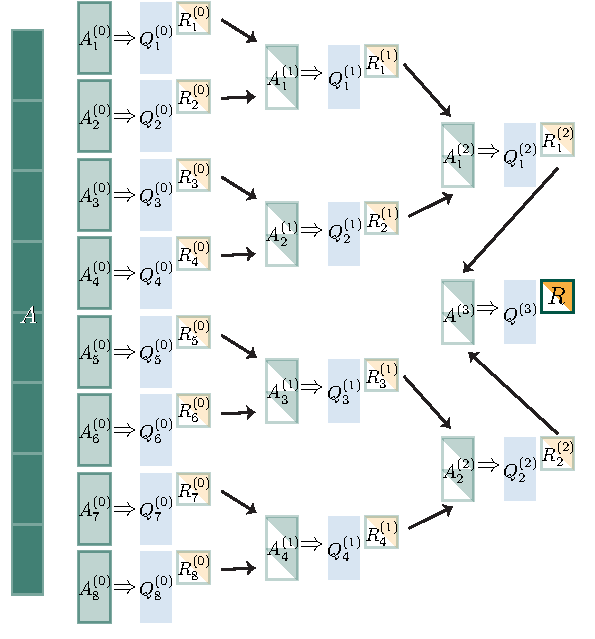
\includegraphics{./figures/TSQR.pdf}
%			\caption{\label{fig:TSQR} Visualization of the TSQR factorization (AllReduce) algorithm.}	
%		\end{figure}
		
		%\subsubsection{Variants of TSQR}
			


%Since the subroutine with leading order FLOPs of an HQR implementation is the dot product, and we will use it to approximate the computational complexity of the TSQR algorithm.
%For a tall-and-skinny matrix $\bb{A}\in\R^{m\times n}$ where $m\gg n$, the deepest possible TSQR scheme has $\lfloor\log_{2}(\frac{m}{n})\rfloor$ levels of recursion. 
%The general idea is that deeper levels of recursion lead to shorter dot products, but more FLOPs over all, and both of these factors contribute to the accumulation of rounding errors and its effect on the accuracy of the QR factorization.
\begin{theorem}
	\label{thm:moriTSQR}
	Let $\bb{A}\in\R^{m\times n}$ with $m\geq n$ have full rank, $n$, and $\hat{\bb{Q}}\in\R^{m\times n}$ and $\hat{\bb{R}}\in\R^{n\times n}$ be the thin QR factors of $\bb{A}$ obtained via Algorithm~\ref{algo:par_tsqr}. 
	Then we have normwise forward error bounds
	\begin{align*}
	\hat{\bb{A}} = \bb{A} +\bb{\Delta A} &=  \bb{Q}(\bb{R} + \bb{\Delta R}),\\
	\hat{\bb{Q}} &= \bb{Q} + \bb{\Delta Q},
	\end{align*}
	where
	\begin{align}
	\|\bb{\Delta R}\|_F, \|\bb{\Delta A}\|_F &\leq \left[n\tilde{\gamma}_{ \frac{m}{2^L}}+(1+n\tilde{\gamma}_{ \frac{m}{2^L}})\left\{(1+n\tilde{\gamma}_{ 2n})^L-1\right\}\right]\|\bb{A}\|_F, \text{ and} \label{eqn:tsqrRA}\\
	\|\bb{\Delta Q}\|_F &\leq \sqrt{n}\left[(1+n\tilde{\gamma}_{ \frac{m}{2^L}})(1+n\tilde{\gamma}_{ 2n})^L -1\right].\label{eqn:tsqrQ}
	%& \leq \left[n\tilde{\gamma}_{ \frac{m}{2^L}}+(1+n\tilde{\gamma}_{ \frac{m}{2^L}})\left\{(1+n\tilde{\gamma}_{ 2n})^L-1\right\}\right]\|\bb{A}\|_F,\label{eqn:tsqrA}
	\end{align}
	Furthermore, if we assume $n\tilde{\gamma}_{ \frac{m}{2^L}}, n\tilde{\gamma}_{ 2n} \ll 1$, the coefficient for $\|\bb{A}\|_F$ in Equations~\ref{eqn:tsqrRA} can be approximated as
	\begin{equation}
	\left[n\tilde{\gamma}_{ \frac{m}{2^L}}+(1+n\tilde{\gamma}_{ \frac{m}{2^L}})\left\{(1+n\tilde{\gamma}_{ 2n})^L-1\right\}\right] \simeq n\tilde{\gamma}_{ \frac{m}{2^L}} + Ln\tilde{\gamma}_{ 2n}, %(46) in Mori
	\end{equation}
	and the right hand side of Equation~\ref{eqn:tsqrQ} can be approximated as
	\begin{equation}
	 \sqrt{n}\left[(1+n\tilde{\gamma}_{ \frac{m}{2^L}})(1+n\tilde{\gamma}_{ 2n})^L -1\right]\simeq \sqrt{n}\left(n\tilde{\gamma}_{ \frac{m}{2^L}} + Ln\tilde{\gamma}_{ 2n}\right). %(67) in Mori
	\end{equation}
	We can also form a backward error, where $\bb{A}+\bb{\Delta \bb{A}_{\text{TSQR}}} = \hat{\bb{Q}}\hat{\bb{R}}$, and both $\hat{\bb{Q}}$ and $\hat{\bb{R}}$ are obtained via Algorithm~\ref{algo:par_tsqr}.
	Then,
	\begin{equation}
	\|\bb{\Delta \bb{A}_{\text{TSQR}}}\|_F =\|\bb{Q \Delta R} + \bb{\Delta Q}\hat{\bb{R}}\|_F \simeq \sqrt{n}\left(n\tilde{\gamma}_{ \frac{m}{2^L}} + Ln\tilde{\gamma}_{ 2n}\right)\|\bb{A}\|_F.
	\end{equation}
\end{theorem}

In Section~\ref{sec:mpupHQRcomparison}, the steps of the HQR algorithm resulted in an error bound of  $\mathcal{O}(\epsilon)$, where the constant is some function with respect to $n$ and where $\epsilon$ is the error bound for a single Householder transformation, described in Equation~\ref{eqn:applyPgen} .
% MATH QUESTION: Can n\epsilon and n^{3/2}\epsilon both be considered as O(\epsilon)?
Similarly, the analysis behind Theorem~\ref{thm:moriTSQR} can be generalized via defining $\epsilon_1$ to be the error bound for a single Householder transformation corresponding to the vector length at the initial level $0$, $\frac{m}{2^L}$, and defining $\epsilon_2$ to be the error bound for a Householder transformation corresponding to vector length in all deeper levels,  $2n$.
This generalization leads to the error bound coefficients
\begin{align}
 n\epsilon_1 + Ln\epsilon_2& \qquad\text{for}\quad  \|\bb{\Delta Q}\|_F, \|\bb{\Delta \bb{A}_{\text{TSQR}}}\|_F,\\
 \sqrt{n}(n\epsilon_1+Ln\epsilon_2)& \qquad\text{for}\quad \|\bb{\Delta R}\|_F, \|\bb{\Delta A}\|_F.
\end{align}

In a uniform-precision setting, these correspond to
\begin{equation}
\epsilon_1 = \tilde{\gamma}^{(\frac{m}{2^L})}\quad \text{and}\quad \epsilon_2 = \tilde{\gamma}^{(2n)},
\end{equation}
and in the mixed-precision setting outlined in Assumption~\ref{assump:mp}, they correspond to
\begin{equation}
\epsilon_1 = \gamma_w^{(6d_1+6z+13)}, \quad \text{and } \epsilon_2 = \gamma_w^{(6d_2+6z+13)},
\end{equation}
where $d_1 := \lfloor{(\frac{m}{2^L}-1)\frac{u_s}{u_w}\rfloor}$ and $d_2 :=\lfloor \frac{(2n-1)u_s}{u_w}\rfloor$ respectively.
In both settings, we see that increasing $L$ may decrease $\epsilon_1$, but may still increase the overall bounds; the larger $L$ still could have an adverse effect on the coefficients in Theorem~\ref{thm:moriTSQR}.
This trade-off is precisely the balance between the sizes of initial blocks and the number of levels in the TSQR algorithm, and an optimal TSQR scheme would ideally minimize $\epsilon_1$ and $\epsilon_2$ with the choice of $L$.
These error bounds are studied in detail in the following section. %Section ~\ref{sec:HTSQR}.
%, resulting in some sort of a trade-off balance between , 
%While the original problem required forming the QR decomposition of a $m$-by-$n$ matrix, an $L$-level TSQR solves $2^L$ QR factorizations of $\lfloor\frac{m}{2^L}\rfloor$-by-$n$ matrices in Level $0$, followed by $2^{L-1}, \cdots, 2^{0}$ QR factorizations of $2n$-by-$n$ matrices in levels $1$ to $L$, which sums to $2^{L}-1$ QR factorizations of $2n$-by-$n$ matrices. 

\subsubsection{HQR and TSQR error bound comparison}
\label{sec:HTSQR}
We compare the error bounds for HQR and TSQR algorithms. 
\paragraph{Uniform precision comparison}Consider the larger error bounds in the uniform precision equivalents of Theorems~\ref{thm:feHQR} and \ref{thm:moriTSQR}, which are the bounds of $\bb{\Delta Q}$ and $\bb{\Delta A}$. 
In order for the a meaningful TSQR error bound to outperform the bound for the HQR algorithm, we need integers $m, n > 0$, and $L\geq0$ such that,
\begin{equation*}
1\gg n^{3/2}\gamma^{(m)} \gg n^{3/2}(\gamma^{(\frac{m}{2^L})}+L\gamma^{(2n)}).
\end{equation*}
If we assume $\frac{m}{2^L}=2n$, the HQR bound is $\frac{L+1}{2^L}$ larger than the bound for TSQR with $L$ levels. 
For example, in single precision, a HQR of a $2^{15}$-by-$2^6$ matrix results in an upper bound relative backward error ($\|\bb{A}-\hat{\bb{Q}}\hat{\bb{R}}\|_F/\|\bb{A}\|_F$) of $\approx${\tt1.002}, but a TSQR with $L=8$ is bounded by $\approx${\tt 3.516e-02}. 
This case exemplifies a situation in which stability is not guaranteed in HQR, but the method is stable when using TSQR, even in the worst-case. 
Now consider some $2^{20}$-by-$2^{12}$ matrix and QR factorizations performed with double precision.
The error bound for HQR is {\tt 1.686e-7}, whereas the error bound for TSQR with 12 levels is {\tt 5.351e-10}.
In general, we can conjecture that values of $L$ that can make $m2^{-L}$ and $2Ln$ much smaller than $m$, should produce a TSQR that outperforms HQR in worst-case scenarios, at least in uniform precision settings.
However, the range of matrix sizes that TSQR can accommodate decreases as $L$ grows larger.
%, and the range is only half of that of HQR even for a single-level TSQR. 
Figure~\ref{fig:paramspace} shows the matrix sizes HQR, 2-level TSQR, and 4-level TSQR can accommodate as well as their respective error bounds.\par
\begin{wrapfigure}{l}{.45\textwidth}
	\centering
	%\vspace{-15pt}
	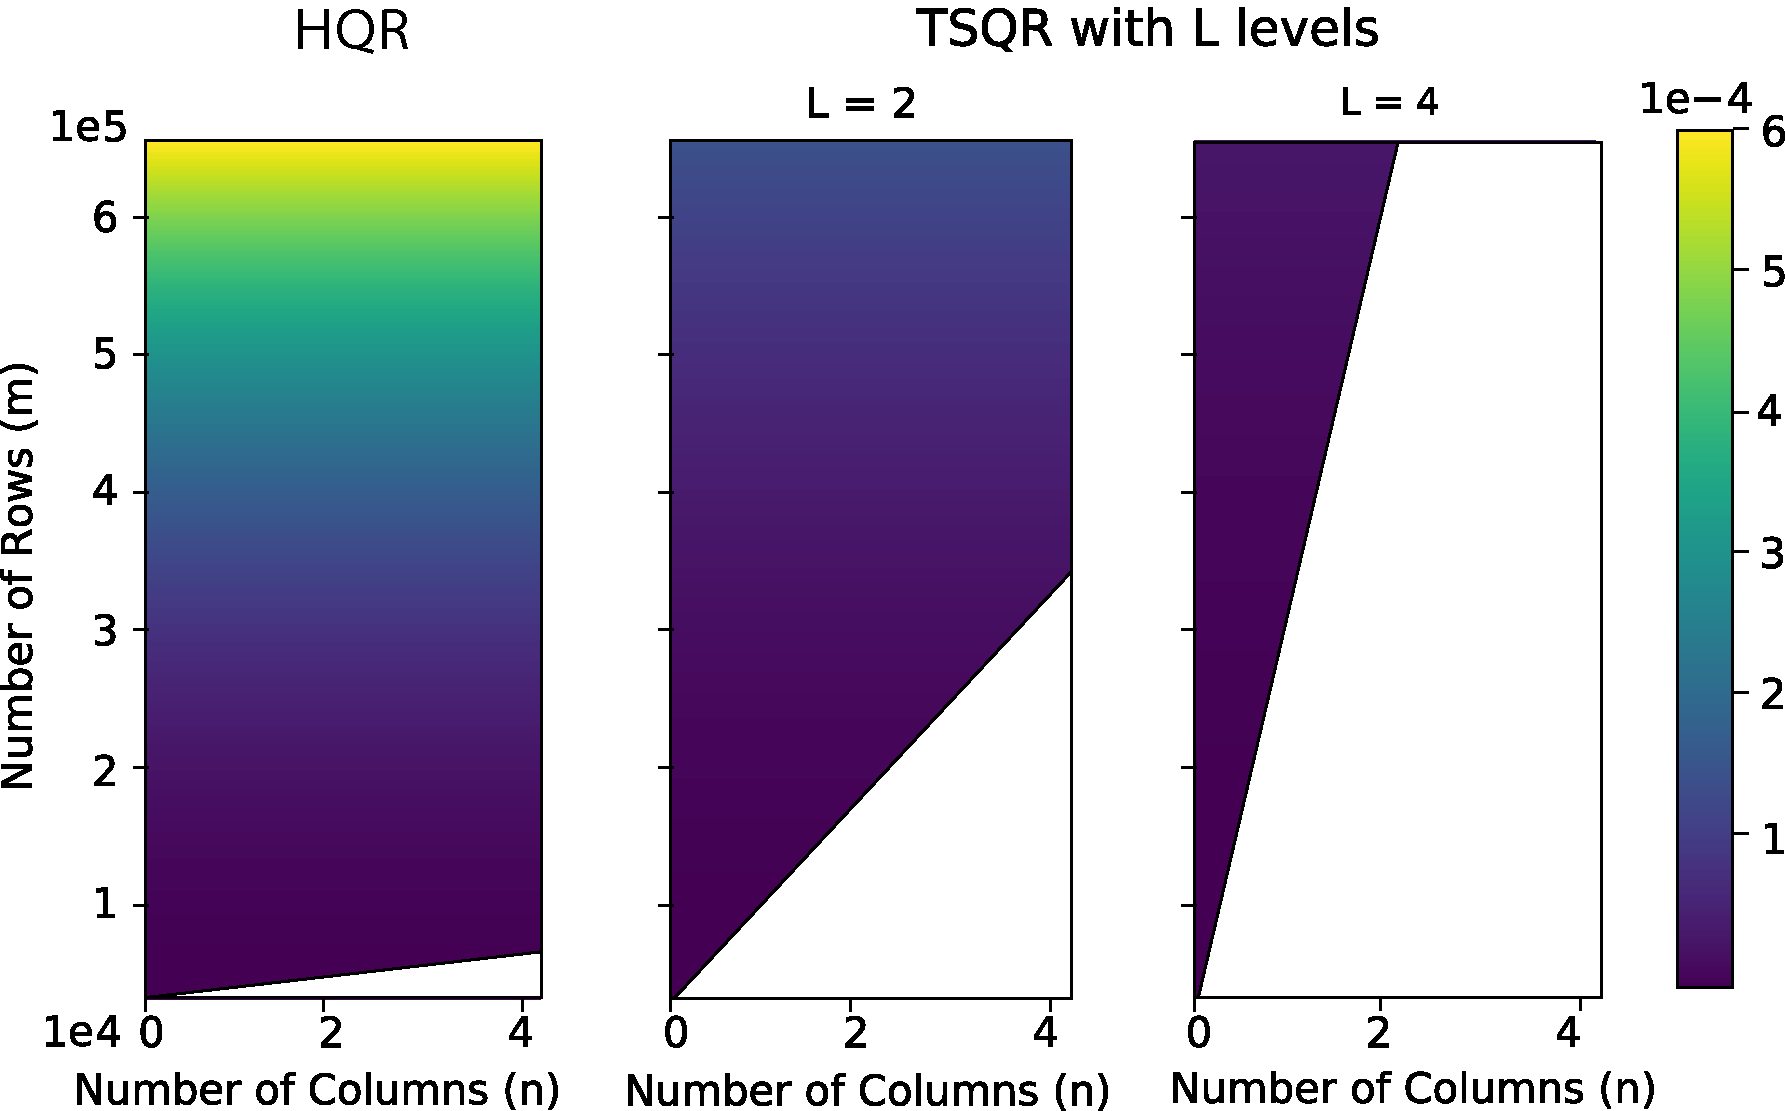
\includegraphics[width=.45\textwidth]{./figures/paramspace.png}
	\caption{\label{fig:paramspace} Non-white space indicates allowable matrix sizes for each scheme, and color map represents error bounds for $\|\bb{\Delta Q}\|_F$ for uniform precision error analysis when using double precision arithmetic.}
	\vspace{-10pt}	
\end{wrapfigure}
\paragraph{Mixed precision comparison}Consider a mixed-precision setting such as in Assumption~\ref{assump:mp}, and we assume $u_p=u_w$, so that $z=2$.
In order for the a meaningful TSQR error bound to outperform the bound for the HQR algorithm, we now need integers $m, n > 0$, and $L\geq 0$ such that
\begin{equation*}
1\gg n^{3/2}\gamma_w^{(6d + 25)} \gg n^{3/2}(\gamma_w^{(6d_1+ 25)}+L\gamma_w^{(6d_2+ 25)}),
\end{equation*}
where $d=\lfloor\frac{(m-1) u_s}{u_w}\rfloor$, $d_1 = \lfloor{(\frac{m}{2^L}-1)\frac{u_s}{u_w}\rfloor}$, and $d_2 =\lfloor \frac{(2n-1)u_s}{u_w}\rfloor$. 

In contrast to the analysis for uniform precision settings, large $L$ values do not necessarily reduce the error bounds of TSQR. 
While large $L$ can imply $m\gg m2^{-L}+2Ln$, it does not always lead to $d \gg d_1+Ld_2$.
Although the theoretical error bounds do not give a clear indication of the worst-case performances of HQR and TSQR in mixed-precision settings, TSQR outperformed HQR on ill-conditioned matrices within our numerical simulations.

These experiments are discussed in detail in the next section.%Section~\ref{sec:NE}.



\subsection{Numerical Experiment}
\label{sec:NE}
%\subsection{Single Precision}
In Section~\ref{sec:HTSQR}, we theorized that conditions exist where TSQR could outperform HQR and that these conditions were hard to identify in mixed-precision settings. 
An empirical comparison of these two QR factorization algorithms in double precision can be found in \cite{Mori2012}, where they conclude that deeper TSQR tends to produce more accurate QR factorizations than HQR.
However, using TSQR with deep levels (large $L$) can actually start to perform worse than TSQR with shallower levels (smaller $L$), since deeper levels require more FLOPs.
We instead focused on comparing HQR and TSQR performances in a mixed-precision setting.
Our numerical simulations show that TSQR can still outperform HQR in low, mixed-precision settings in practice even though the theoretical bounds do not guarantee stability.
%are all $\mathcal{O}(10)$ (c.f. Table~\ref{table:HTSQRerr}), and get larger as we go from HQR to TSQR, and larger as we increase $L$. 
Our empirical results do not behave as the theoretical bounds suggest, and even show opposite trends at times. 
This discrepancy highlights the shortcomings of deterministic error bounds that are too pessimistic. \par
%showed that there exists conditions in which the worst-case rounding error bound for TSQR can be expected to be smaller than that of HQR. 
%These conditions are met more easily in high, uniform-precision settings than low mixed-precision settings.
%The success of TSQR in high, uniform-precision settings is explored and discussed in \cite{Mori2012}, where they conclude that the computed relative error, $\|\hat{\bb{Q}}\hat{\bb{R}}-A\|_F$, tends to decrease as they increase $L$, but only up to a certain point.
%This may appear to contradict our conclusion in Section~\ref{sec:upHTSQR}, where we found that as long as $\frac{L}{2^{L-1}}\ll 1$, there e 
%\subsubsection{Experiment Details}
We used Julia v1.0.4 for all of the numerical simulations. 
This programming language allows half precision storage as well as {\tt castup} and {\tt castdown} operations to and from single and double precisions, but has no half precision arithmetic.
Therefore, we relied on using Algorithm~\ref{algo:simulate} for $f\in \text{OP} \cup\{{\tt dot\_product}\}$ to simulate half and mixed-precision arithmetic operations. 
%Specifically, we approximated , and 
%To simulate the mixed-precision setting described in Assumption~\ref{assump:mp} with $u_p = 0$ (which implies $z=1$), we used Algorithm~\ref{algo:simulate} for the dot product routine.
%That is, for $\bb{x}_{\text{half}},\bb{y}_{\text{half}}\in\F_{\text{half}}^m$, we approximated $\fl(\bb{x}_{\text{half}}^{\top}\bb{y}_{\text{half}})$ with {\tt simHalf}$(${\tt dot\_product} $, \bb{x}_{\text{half}}, \bb{y}_{\text{half}})$ to simulate mixed-precision dot products.
%We used Algorithm~\ref{algo:simulate} for all other operations as well to simulate half precision arithmetic.
For HQR, we created a mixed-precision version of the LAPACK routine xGEQRF, where the dot product subroutine was approximated by $\fl(\bb{x}_{\text{half}}^{\top}\bb{y}_{\text{half}})$ with {\tt simHalf}$(${\tt dot\_product} $, \bb{x}_{\text{half}}, \bb{y}_{\text{half}})$ to simulate the mixed-precision setting described in Assumption~\ref{assump:mp} with $u_p = 0$ (which implies $z=1$), and we used Algorithm~\ref{algo:simulate} on all other basic operations in OP to simulate half/storage precision arithmetic. 
%Using these simulated operations as subroutines for 
%By using these simulated half and mixed precision versions of basic operations at subroutines for our implementation of the LAPACK routine xGEQRF, we 
%To implement half and mixed-precision simulations within HQR, we wrote our own versions of it that almost replicates LAPACK routine xGEQRF, where the disparity only comes from the storage format of the information required to build the $\bb{Q}$ factor. 
This HQR was then used as a subroutine of TSQR as well. 
There are cases where the rounding will differ between the mixed-precision setting and the way we mimic it, i.e., basic operations that are meant to be in half/storage precision arithmetic, but are instead casted up to single and back down, as the tiebreaker within correct rounding may lead to different results than true half/storage precision arithmetic. 
All in all, our experiments nearly replicated the mixed-precision setting we assumed for the error analysis in Sections~\ref{sec:HQRre} and \ref{sec:TSQRre}.\par 
%Although we kept the matrix size constant, we varied the condition numbers of these matrices by the method described below.
%We speculated that matrices with larger condition numbers would behave closer to the ``worst-case scenario'' with respect to rounding errors.
%Table~\ref{table:HTSQRerr} shows the theoretical error bounds from Section~\ref{sec:HQRre} and \ref{sec:TSQRre} that correspond to the conditions of our experiment.
%Stability is not guaranteed for any of these QR factorization methods. 
%
%\begin{table}[h]
%	\centering
%	\begin{tabular}{||c|c|c|c|c|c|c|c||} 
%		\hline
%		$L$ & $0$ & $1$ & $2$ & $3$ & $4$ & $5$ & $6$ \\ \hline
%		$n^{3/2}(\gamma_w^{(6d_1+ 25)}+L\gamma_w^{(6d_2+ 25)})$ & {\tt 9.36} & {\tt 18.73} & {\tt 28.09} & {\tt 37.46} & {\tt 46.82} & {\tt 56.19} & {\tt 65.55}\\ \hline
%	\end{tabular}
%	\caption{Error bounds for when $m=4000$, $n=100$, $u_w=u_{\text{half}}$, $u_s={\text{single}}$, and $d_1,d_2$ are defined in Section~\ref{sec:TSQRre}. Error bound for HQR is recovered when $L=0$.}
%	\label{table:HTSQRerr}
%\end{table}

%\paragraph{Constructing Test Matrices}
Following example from \cite{Mori2012}, we used $m$-by-$n$ random matrices, $\bb{A}_{\alpha}$, constructed via
\begin{equation}
\bb{A}_{\alpha} = \bb{Q'}(\alpha \bb{E} + \bb{I})/\|\bb{Q'}(\alpha \bb{E} + \bb{I})\|_F,
\label{eqn:genRM}
\end{equation}
where $\bb{Q'}\in\mathbb{R}^{m\times n}$ is a random orthogonal matrix and $\bb{E}\in\R^{n\times n}$ is the matrix of $1$'s. 
The random orthogonal matrix $\bb{Q'}$ is generated by taking a QR factorization of an iid $4000$-by-$100$ matrix sampled from $Unif(0,1)$, and we used the built-in QR factorization function in Julia.
By construction, $\bb{A}_{\alpha}$ has 2-norm condition number $n\alpha+1$. 
By varying $\alpha$ from {\tt 1e-4} to {\tt 1}, we varied the condition number from $1.1$ to $101$, and we generated $10$ samples for each value of $\alpha$.

%\subsubsection{Results}


We generated random matrices of size $4000$-by-$100$ using Equation~\ref{eqn:genRM} and computed their HQR and TSQR for $L=1, \cdots, 6$ in a mixed-precision setting that simulates Assumption~\ref{assump:mp} with $z=1$.
The relative backward error, $\|\hat{\bb{Q}}\hat{\bb{R}}-\bb{A}\|_F/\|\bb{A}\|_F$, was computed by casting up $\hat{\bb{Q}}$, $\hat{\bb{R}}$, and $\bb{A}$ to double precision to compute the Frobenius norms.
Note that the mixed-precision HQR error bounds $n\tilde{\gamma}_{w}^{(6d+6z+13)}$ and $n^{3/2}\tilde{\gamma}_{w}^{(6d+6z+13)}$ for $m=4000$ and $n=100$ are {\tt 0.936} and {\tt 9.364} respectively, and the mixed-precision TSQR bounds for $L=1,\cdots, 5$  are even larger, which indicates that our error bounds do not guarantee stability.\par

\begin{wrapfigure}{l}{.4\textwidth}
	\centering
	\vspace{-10pt}
	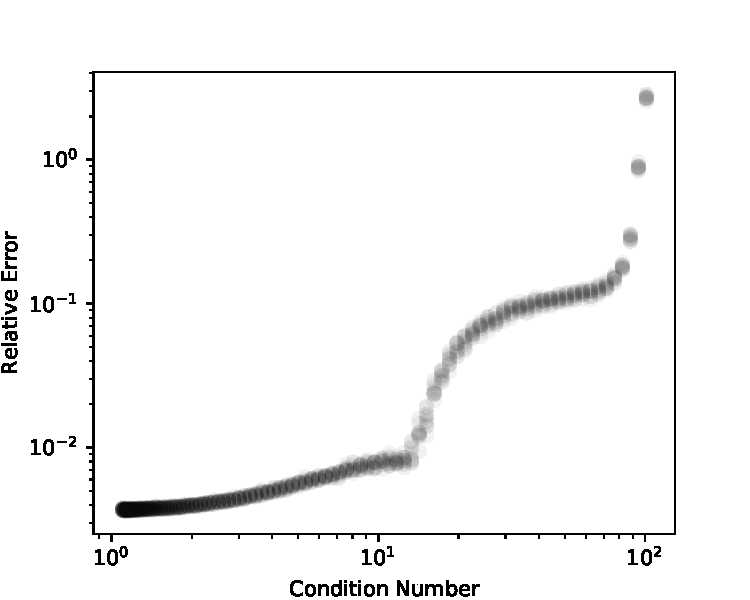
\includegraphics[width=.4\textwidth]{./figures/unblocked.pdf}
	\caption{\label{fig:unblocked} HQR errors for matrices with varying condition numbers.}
	%\vspace{-10pt}	
\end{wrapfigure}
Figure~\ref{fig:unblocked} shows the backward errors of mixed precision HQR increasing as the theoretical condition numbers of the generated random matrices increase, and these errors correspond to the error data on the vertical axis, $L=0$, of Figure~\ref{fig:allTSQR}.
In addition to the errors from HQR, Figure~\ref{fig:allTSQR} shows the errors from mixed precision TSQR of levels varying from $L=1$ to $L=5$, where each line represents the errors of HQR and variants of TSQR calculated from the same random test matrix.
Figure~\ref{fig:allTSQR} reveals two different trends for the errors as we deepen the complexity of the QR algorithm from HQR to TSQR with 5 levels. 
One trend occurs for matrices with smaller condition numbers, where HQR and all levels of TSQR are stable, but deepening the levels of TSQR worsens the errors. 
The other trend occurs for matrices with higher condition numbers, where single-level and 2-level TSQR yield smaller errors than HQR. 
In these cases, TSQR with 3 or more levels have errors similar to or worse than 2-level TSQR, but those errors tend to not rise above the HQR errors.
These results suggests that TSQR can significantly outperform HQR even in mixed-precision settings, and particularly when HQR is unstable due to larger condition numbers.
Although this experiment focused on condition numbers, identifying other properties that point to better performance of TSQR than HQR can further broaden the potential use of mixed-precision TSQR in applications.
%The first trend When the error is low enough for the unblocked QR factorization, TSQR performs worse for these matrices.
%Recall that machine precision for half-precision is about $10^{-3}$. 
%This shows that the traditional QR factorization had been very good to begin with.
%Finally, even when TSQR is \textit{successful} initially, we can see that too many initial blocks can become a problem as well. 
%
%Overall, this figure shows a variety of results that encourage further exploration. 
%We have shown that TSQR can improve on certain matrices where the unblocked HQR algorithm was highly unstable in half-precision.
%Identifying which matrix properties correlate to TSQR and why can help broaden the possibility of using lower precision arithmetic for QR factorizations.

\begin{figure}[h!]%{r}{.53\textwidth}
	\centering
	%\vspace{-10pt}
	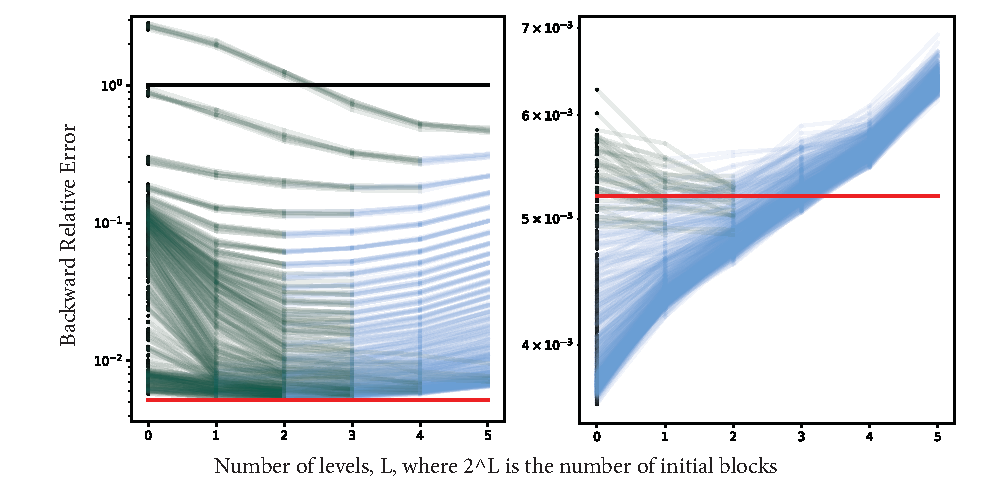
\includegraphics[width=0.8\textwidth]{./figures/allTSQR2.pdf}
	\caption{\label{fig:allTSQR} Left plot shows the relative error of QR factorization for matrices with condition numbers ranging from 5.3 to 101, and the right plot shows the errors for matrices with condition numbers ranging from 1.1 to 5.3. }
	\vspace{-10pt}
\end{figure} 
